\section{Introduction}\label{sec:positioningIntroduction}
A autonomous vehicle has as a main function to control all actors on its own.
This means that no human give a sign to the car that now its the time to turn the motor on.
To decide how the single components have to act at which time 
the car need information about its own position which are as good as possible.
This chapter will present some sensors which can be used to get information about the position and rate them in different categories.
Another part of this chapter is to calculate the most possible current position based on the input data of different sensors.


\section{Sensor Types}
\begin{itemize}
\item absolute sensors
	\subitem lateration
		\subsubitem GPS	
		\subsubitem Mobile telephony
\item environment detection
	\subitem image recognition
	\subitem bumper
	\subitem distance sensor
		\subsubitem ultrasonic
		\subsubitem infrared sensor
\item relative sensors
	\subitem touchless
		\subsubitem gyro sensor
		\subsubitem acceleration
		\subsubitem magnetometer
	\subitem other
		\subsubitem rotary encoder
		\subsubitem mouse sensor
\end{itemize}


\section{Measures Fails, Tolerance, Errors}
\begin{figure}
\makebox[\linewidth]{
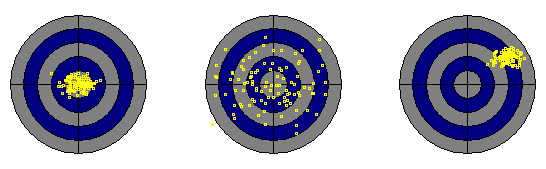
\includegraphics[scale=0.5]{picturesPositioning/precisionDarts.png}
}
\caption{Error Types \cite{img:precisionDarts}}
\label{fig:errorTypes}
\end{figure}
The used sensors have different properties.
One is faster and the another one have a higher precision.
In this section the different types of errors which a sensor can produce are explained.


\subsection{Methodical Errors}
Methodical errors are errors which are expectable.
This means the errors have similar properties.
They occurs mainly when devices are badly calibrated.
A example of a methodical error is the right picture of Errors~\ref{fig:errorTypes}.
This example shows that methodical errors are those which are the easiest one to create an algorithm which calculates the real value.
Such a algorithm could be also a simple addition or multiplication.
Also a calibration of the device can help to improve the result.


\subsection{Run Away Values}
Run away values are single measure results which doesn't fit in the expected range.
This means that most of the values which are measured are close to the real value except a very small count of values.
A very popular example for a run away value are the red pixels in a photo which was made by a digital camera.
Although the most pixel fit very well there are some pixel which return a value which is to much red.
This effect of digital cameras come through when the image sensor get to hot.
However, this effect that heat increase the error rate is not only by image sensors.
Also other sensors produce much more errors if they become hot.
The type of error which is produced through heat can be very different.
Some sensors lose precision other produce a methodical error.
Often sensors produce combined bugs.


\subsection{Brake Down}
A break down is when a sensor lose its full functionally.
The way a brake down can happen could be very different.



\subsection{Bad Precision}


\section{Selection of Sensors}


\section{Combine Different Sensors}


\section{Position Specification}
